\documentclass[10pt,a4paper]{article}
\usepackage[utf8]{inputenc}
\usepackage{amsmath}
\usepackage{amsfonts}
\usepackage{amssymb}
\usepackage{graphicx}

\title{KDD Cup 2013 - Author-Paper Identification Challenge}
\author{ Mike Koeman \and Vincent Slieker   \and Aram Verstegen \and Rob Tiemens}
\graphicspath{./Images/} 

\begin{document}

\maketitle


\begin{abstract}
The ability to search literature and collect and aggregate metrics around publications is a central tool for modern research. Both academic and industry researchers across hundreds of scientific disciplines, from astronomy to zoology, increasingly rely on search to understand what has been published and by whom.

The profile of an author with an ambiguous name tends to contain noise, resulting in papers that are incorrectly assigned to him or her. This KDD Cup task challenges participants to determine which papers in an author profile were truly written by a given author.

We adapted two methods to cope with these problems. We used a text analysis method to create topics. These topics are then treated as new features to classify paper-author combinations. An advanced graph database is used to create a graph from all authors. Examining the relations between authors will reveal useful information to profile a writer.
\end{abstract}

\nocite{chowdhury2010introduction}
\nocite{liu2005co}
\nocite{glanzel2005analysing}
\nocite{morel2009co}
\nocite{niels2008writer}
\nocite{steyvers2004probabilistic}
\nocite{newman2004coauthorship}
\nocite{Liu:2006:WDM:1215470}
\nocite{Witten:2005:DMP:1205860}


\section*{Introduction}

For the course ``Machine Learning in Practice'' we participated in the annual KDD-cup.
This year's KDD-Cup is about author-paper identification.
In this paper we present and discuss our approach to try to win this competition.
The methodology is illustrated using the data provided by the KDD-Cup.
Our approach involves three different methods to find features in the given data set.
We've used a probabilistic author-topic model~\cite{steyvers2004probabilistic} to extract topics from  the data, co-authorship graphs to get extra features from social connections between authors~\cite{liu2005co} and we have used the simple features available from the benchmark example project provided by the competition organisers.
These features are then used together to train a random forest classifier on the labeled data sets, which is then used to make predictions about the unlabeled data sets.

The outline of the paper is as follows: in Section~\ref{sec:background} we describe the scientific background of our methods, then describe our implementation details in Sections~\ref{sec:graph-implementation},~\ref{sec:text-implementation},~\ref{sec:smaller-features-implementation} and \ref{sec:classifier-implementation}. Finally, we present our results in Section~\ref{sec:results}.


\section{Background \label{sec:background}}

\subsection{Social Network Graph Model \label{sec:graph-background}}


We tried to derive the likelihood of a given author contributing to a certain paper by looking at the connections from that author to the other authors contributing to that paper in a social network graph.
In order to determine if and how any two given authors from an unlabeled set are connected to one another, we ideally wanted to extract a measure of probability of any two authors collaborating based on the known data and construct weighted edges between these authors, in order to then find paths in our graph with the lowest weight to serve as a measure of maximum likelihood of co-authorship given the previously known social connections.

We have constructed a graph where all authors from our data set are represented as vertices (nodes) and created directed edges between those based on their common occurrences in the papers of both our training and evaluation data set.
Our idea to model relationships using this representation was directly inspired by the research done by Xiaoming Liu et al \cite{liu2005co}, who describe the chosen representation of the graph and suggest various metrics and classifier algorithms that may operate on it.

Liu et al have specified a way to normalize the weight of a co-authoring relationship between two authors by averaging the measured frequency (sum of a pair's co-authorships weighted by the number other co-authors in those publications) by the summed frequency of the other author's co-authorships.

\begin{align*}
\textbf{Count authors}~
	f(a_k) &= \#authors \\
\textbf{Exclusivity}~
	g_{i,j,k} &= 1 / (f(a_k)-1) \\
\textbf{Co-authorship frequency}~
	c_{i,j} &= \sum_{k=1}^{m} g_{i,j,k} \\
\textbf{Normalized weight}~
	w_{i,j} &= \frac{c_{i,j}}{\sum_{k=1}^{n} c_{i,k}}
\end{align*}

Our recipe for (sparsely) drawing the edges between author vertices and computing their weights based on this method is as follows:


\begin{enumerate}
  \item Create a relationship (edge) between each 2-pair of all authors from each paper (if it doesn't already exist).
  \item Exclusivity: Each of these relationships gets a property of exclusivity, which represents the number of authors on this paper (which by inversion gives a relative exclusivity for their co-authoring relationship within this paper).
  \item Frequency: The sum of these exclusivity values for each relationship over all co-authored papers (which can be aggregated as a single, summing property on the edge for all co-authorships of two connected authors to keep the graph sparse).
  \item Weight (from A to B): The co-authorship frequency between A and B, averaged over the summed frequency of all of B's co-authorships.
\end{enumerate}

If it requires over 4 steps to connect one author to another by only using this co-authorship path it should be considered a large distance under the assumption that familiar people have at least cooperated once before or have at least one common coauthor resulting in a distance of respectively one and two.
It is also shown by Erd\"os numbers that the number of steps that have to be taken from one to another is likely to be very limited resulting a quadratically scaled probability \cite{balaban2002co}.


\subsection{Text Analysis Model \label{sec:text-background}}



For the use of text-analyses, we read the paper "Probabilistic author-topic models for information discovery". This model is already used in the KDD-cup of 2013. The author-topic model creates a number of topics in which to classify the papers.  \cite{steyvers2004probabilistic}. The model not only discovers what topics are expressed in a document, but also which authors are associated with each topic. To simplify the representation of documents, the authors use a bag of words assumption that reduces each document to a vector of counts, where each vector element corresponds to the number of times a term appears in the document \cite{chowdhury2010introduction}. Each author is associated with a multinomial distribution over topics. A document with multiple authors has a distribution over topics that is a mixture of the distributions associated with the authors. When generating a document, an author is chosen at random for each individual word in the document. This author picks a topic from his or her multinomial distribution over topics, and then samples a word from the multinomial distribution over words associated with that topic. This process is repeated for all words in the document. In the model, the authors produce words from a set of $T$ topics. When $T$ is kept relatively small relative to the number of authors and vocabulary size, the author-topic model applies a form of dimensionality reduction to documents. Topics are learned which capture the variability in word choice across a large set of documents and authors. 

\begin{figure}
\begin{center}
	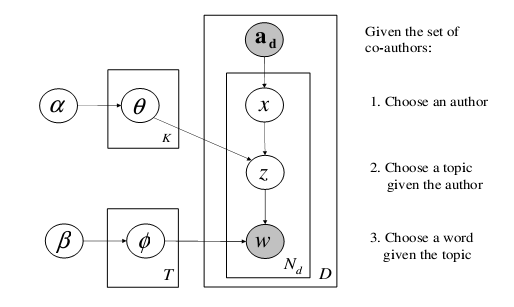
\includegraphics[scale=1]{./Images/model.png}
	\caption{The graphical model for the author-topic
model using plate notation.\cite{steyvers2004probabilistic} \label{fig:model}}
\end{center}
\end{figure}

Figure \ref{fig:model} illustrates the generative process with a graphical model using plate notation. In the author-topic model, observed variables not only include the words $w$ in a document but also the set of coauthors $A_d$ on each document $d$. Currently , the model does not specify the generative process of how authors choose to collaborate. Instead, the authors assume there is a co-author graph available. We create the graph in section ...

@todo sectie erbij.




\section{Co author graph \label{sec:graph-implementation}}

We have constructed a co-authorship graph model using the Java Universal Network/Graph (JUNG) Framework, an open-source Java library \cite{o2005analysis} and explored the possibilities of using the Neo4j graph database software \cite{rodrigez2010mysql} in search of better performance of our model with such a large data set.

The first features included were only related to a given author, like for instance their number of co-authors (the number of outgoing connections) or the number of papers they have written.
In order to determine the likelihood of two authors collaborating we wanted to use the (weighted) Dijkstra distance between two authors.
We chose to use the Dijkstra distance as our basic measure because it works even with unweighted connections between authors and gives a reasonable indication of whether two authors are at least familiar to one another \cite{o2005analysis}.
If it requires over 4 steps to connect one author to another by only using this co-authorship path it should be considered a large distance under the assumption that familiar people have at least cooperated once before or have at least one common coauthor resulting in a distance of respectively one and two.
It is also shown by Erdős numbers that the number of steps that have to be taken from one to another is likely to be very limited resulting a quadratically scaled probability \cite{balaban2002co}.

We used the Dijkstra shortest path algorithm to extract a feature of average and median shortest path distance between a given author and all other authors of that paper.
This results in a measure of how near the author is to any other author who worked on that particular paper.
During experimentation, many measurements of this distance resulted in the value zero or one (suggesting a collaborative  relationship with at least one other coauthor or no connections), so we devised several variations on this feature.
Such a variation was a feature that counted the total number of times a specific author in a given paper had collaborated with a single co-author.
If our Dijkstra distance would result in the value one, we would count the number of papers in which that distance would also equal one.
This gave us an indication of how strong the connection is between two authors that collaborated frequently.

We built our graph based on the complete provided author/paper data set because it presents us with the largest base of what we assume is mostly-reliable information.
We considered the occurrence of co-authorships incorrectly ascribed to any two authors to be limited, and that the overall co-authorship network is still usable even with such relative `noise' added to the graph.
The benefit of including the training set was that it increases the connectedness of our graph, which proved to be a limiting factor in deriving co-authorship probabilities from our graph early on.
We observed that on average over nine out of ten random author pairs were unable to connect through any path between the two vertices.
After including the full data set, low connectivity was still problematic albeit to a lower degree.
When evaluating author pairs in the graph we took into account that the evaluation data set was included and compensated for this by removing the edges between the vertices of the pair of authors that were being evaluated if those were created from the evaluation data set.
We constructed our graph to be sparse and to have directed edges which we attempted to assign weights to later on.
For our first set of simple features this was not necessary. 

The features described so far do not take into account the weight of relative coauthorship frequency between authors as described by Liu et al [4].
We should establish such a measure because an author that produces many papers is more likely to have a collaboration with a randomly selected author than an author who produces only rarely.
At this point we ran into (time and memory-related) trouble because there exists a very large number of pairwise author combinations for which we want to calculate exclusivity/frequency and the resulting normalized weight.
The problem stems from the way in which the modeled co-authorships relate to our graph structure.
We need to construct relationships (with an exclusivity property) for every $n \choose 2$ pairs of authors of every paper with $n$ authors, in two directions.
If that wasn't enough, we would then like to compute the frequency for each relationship by doing aggregates for every such relationship and finally aggregate these aggregates in second-order queries for every single relationship to compute their weight (quadratic).
This becomes quite problematic as the number of authors of a paper grows, and we concluded neither PostgreSQL, MySQL nor JUNG were really the right tools for this job.
As some of the papers feature more than 100 authors this was fast becoming an intractable problem.

We considered simply omitting papers with more than 10 or so reported authors from the weight calculation, but were concerned that this might discard too much valuable information.
After all, it might just be that specifically these `problematic' papers would provide us with highly connected author nodes which function as interconnection `hubs', to better connect otherwise unplaceable authors.

To further investigate the possibility of applying Liu et al's model, which we expected to be computationally heavy but not infeasible (and highly parallelizable) in the time/hardware we had, we turned to the Neo4j software package for graph databases.

Neo4j is a so-called graph database, a type of data storage which differs from conventional relational databases by representing data models not as tables but as property graphs, i.e. a graph in which the nodes and edges have some saved properties.
It features a built-in query language called Cypher, which is somewhat similar to SQL and can be used to traverse the graph and query its properties.
The software boasts useful features like transactional operations, high speed, scalability, availability and consistency.

\begin{verbatim}
START author=node({author_id:42})
MATCH (author)-[coauthorship]->(coauthor)
WITH author,COUNT(coauthorship) as sum
SET author.coauthorships = sum
RETURN author
\end{verbatim}

While this is certainly an enabling technology for this kind of research, we ran into some unexpected scaling problems when trying to apply Liu's model to the KDD cup data set.
While we are newcomers to the technology, we sought to apply it as best we did understand it using the available resources from the project.

The issues that led us to cancel our excursion into Neo4j later on:

\begin{enumerate}


\item[1] The query language interpreter appears to lack an optimizer which parallelizes aggregate operations (in our case: summing values) over paged results, leading to aggregators running in a single thread and attempting to return the full aggregate in one thread context rather than applying something like a map/reduce pattern internally - this eventually leads to memory exhaustion.
We devised our own aggregator using pagination, but did so from outside the Neo4j context.
The performance still proved unsatisfactory but eventually managed to compute the co-authorship frequencies for all relationships as properties on the edges.
The aggregate also seemed to not stay cached, but even when we did cache the aggregate values (by saving them to the related edge as a property) performance was still below our expectations.
Later on we realized this is partly due to the nature of the aggregation itself - no traversed properties are ever re-used after frequencies are computed.

\item[2] The software's multi-threading model is a basic producer/consumer pattern, but there is no built-in option to use more than one producer thread.
	On fast many-core machines, this leads to consumer threads whose workloads are exhausted sooner than they can be appointed new work by the producer, leading to poor multicore performance.
\end{enumerate}
Because at this point we did start to fear this approach to the problem might be practically infeasible for the given case, we started exploring other graph features that were lighter to compute at the last minute before the competition would close, but then decided we should rather use our basic graph features from the JUNG project instead and begin work on submissions.
Given the time invested in this one approach we had hoped to gain more usable features, but certainly still see possibilities of applying the method of social network analysis to the proposed problem.
With our efforts we were able to get to step 3 of our 4-step recipe: we managed to construct co-authorship relationships between any two authors for all paper/author combinations in the given data set with high efficiency (completing in minutes on a cheap multicore Atom netbook) using Neo4j and apply step 3 in a about a day on the same hardware.
Step 4 of our recipe is understandably the most computationally expensive (quadratic), and the performance issues we encountered in Neo4j that prevented us from using faster/bigger hardware caused us to finally abandon the chosen approach.
We suspect that the low interconnectedness we observed was due to the fact that the competition data set was extracted from a larger data set and we appear to have lost the interconnectedness we would expect to see in a real world social network.
We regret to not have considered (as other participating teams did) ways to augment the known connections between authors by linking them through other relationships such as mutual contributions to the same journal or conference, but the $n$ in our $n \choose 2$ relationships would generally become even larger.



\section{Text analyses \label{sec:text-implementation}}

\subsection*{Text analyses \label{sec:imp-text}}

In section \ref{sec:text-background} we introduced a model to create topics from a large collection of text. We adjusted that approach to the problem we needed to solve. We did not have a lot of text from each of the papers. From each paper we only know the title and keyterms. We did not choose to use the keyterms. The keyterms contained a lot of bias and parsing the keyterms in a usable format proved to be difficult. We instead used the titles of the journal or conference the paper was published in. This method has two advantages:

\begin{itemize}
\item[1] we have more terms to identify a paper.
\item[2] More terms are related to each other. If for example the "Automatic detection of acute bacterial pneumonia from chest X-ray reports" was published in a journal congaing the terms "machine learning",  machine learning and X-ray are related. 
\end{itemize}

We now have an sentence $s$ describing the content of paper $p$. Next, all the diacritics, stopterms (in multiple languages), interpunction and double terms are removed from sentence $s$. This saves a lot of entries in the dictionary\cite{chowdhury2010introduction}. After processing sentence $s$, all terms that co-occur in the same sentence are counted and the result is stored in matrix $M$. A short example with some of the terms in sentence $s$ is worked out in tables \ref{tab:before} and \ref{tab:after}.

\begin{table}
	\begin{center}
	

\begin{tabular}{|l|l|l|l|l|}
\hline
	 	& acute  & learning & machine &  x-ray \\ \hline
acute 	&	0 	& 	1 &	 2 &  0	 \\ \hline
learning&	1	&	0 &	 3 &  0	 \\ \hline
machine &	2	&	3 &	 0 &  0	 \\ \hline
x-ray	&	0	&	0 &	 0 &  0	 \\ \hline

\end{tabular} 
	\end{center}
\end{table}


\begin{table}
	\begin{center}

\begin{tabular}{|l|l|l|l|l|}
\hline
	 	& acute  & learning & machine &  x-ray \\ \hline
acute 	&	0 	& 	2 &	 3 &  1	 \\ \hline
learning&	2	&	0 &	 4 &  1	 \\ \hline
machine &	3	&	4 &	 0 &  1	 \\ \hline
x-ray	&	1	&	1 &	 1 &  0	 \\ \hline
\end{tabular} 

	\end{center}
\end{table}

Note that matrix $M$ is symmetric and very sparse. We used this to our advantage and stored this matrix efficiently.


\subsubsection*{Clustering}

In the previous subsection we created matrix $M$. Each row is a separate vector $v$ containing information form which terms co-occurs with a another term. Each vector $v$ is then clustered into one of the $c$ clusters with k-means. In our case, we choose  $c = 20$. The number 20 is a wild guess. In the original paper \cite{steyvers2004probabilistic}, the authors use 300 clusters, but our computers were not able to process that number of clusters. Each cluster now contains terms that co-occur a lot. We call a cluster a topic, just as the original paper. As a distance measure we choose \emph{cosine similarity}. Cosine similarity measures the distance between two vectors. The cosine similarity has a big advantage over the Euclidean distance \cite{chowdhury2010introduction}.  

Not that the authors use EM to cluster matrix $M$. This gives the authors a probability of each term for each cluster. because we used k-means we do not have that information anymore. We only which term is in a certain cluster. In our case, each term can only be in a single cluster.

\subsubsection*{Scoring}

At this point we have 20 clusters. Each cluster $c$ contains several terms that that form a single topic. We then score each paper-author combination against the topics. For each  paper-author combination we created sentence $s$ just as in section \ref{sec:imp-text}. For each term in sentence $s$ we counted the number of occurrences in a topic. This is then used as latent variable for classifying paper-author couples.
\[ \delta_c(t) =\left\{ \begin{matrix} 1 & \mbox{if t is present in c} \\ 0 & \mbox{otherwise} \end{matrix} \right.\]

\[ score_c = \sum_{t \in s} \delta_c(t) \]

\subsubsection*{Optimizing with Tf-Idf}

Thus far, scoring has hinged on how much a term occurs. Common words have a higher score and contribute more towards the final classification. But common words do not say a lot about each sentence\cite{chowdhury2010introduction}. To compensate the higher score for common terms we use a information retreival technique called TF-IDF. Instead of just counting the number of occurrences of a term in a cluster, we assign a TF-IDF for each term and add those together. We simplified TF-IDF for our own use. because a term can only be present once each sentence, we only use IDF. The score for each cluster is now computed as:

\[ \gamma_c(t) =\left\{ \begin{matrix} \mbox{Tf-Idf}(t) & \mbox{if t is present in c} \\ 0 & \mbox{otherwise} \end{matrix} \right.\]


\[ score_c = \sum_{t \in s} \gamma_c(t) \]


\section{Smaller features \label{sec:smaller-features-implementation}}

The data from this also contained smaller, easier to extract, features. The features we also found for \textit{every} paper-author combination.

\begin{itemize}
\item[]Dates. For each author we also include
\begin{itemize}
\item[] First year. The first year the author published a paper. We only looked for papers with a year greater then 1800. All years below are considered bias.
\item[] Last year. The last year the author published a paper. We only looked for papers with a year lower then 2013. All years above are considered bias.
\item[] Average year. Weighted average of all the years the author published a paper.
\item[] Standard deviation of all years
\end{itemize}
\item[] Number of papers written
\item[] Number of journals published in 
\item[] Number of conferences
\end{itemize}


\subsection{Classifying the authors and papers \label{sec:classifier-implementation}}

For our final submission we used two sets of data with the following columns.

\begin{itemize}
\item [] AuthorID 
\item [] PaperID 
\item [] $score_1 \cdots \cdots score_{20}$ 
\item [] First year 
\item [] Last year 
\item [] Average year 
\item [] Average group size
\item [] Number of authors in paper
\item [] Year Standard deviation 
\item [] Number of papers written
\item [] Number of journals published in 
\item [] Number of conferences
\end{itemize}

We only used the valid set to train our classifier. After we trained the classifier we applied the classifier to the test set. because the classifier also gives a probability we used that to rank the outcome.






\section{Results \label{sec:results}}

Below are the results we got when trying different features

\begin{itemize}
	\item[] \textbf{Benchmark only}: 0.86
	\item[] This is the benchmark from Kaggle. We wrote the same code only in C\# instead of python. This was our final score.
	\item[] \textbf{Topics only}: 0.60
	\item[] In this submission we only used our paper-topic model with no classifier. This approach did not score very well. Using IDF to normalize the the vector improved our score a bit (0,02). Comparing the means of deleted papers and comfirmed papers showed a difference of a little over one standar deviation  
	\item[] \textbf{Graph, year features and benchmark}: 0.78
	\item[] The graph features found using our graph search algorithms.
	\item[] \textbf{Year features and  benchmark}: 0.86
	\item[] Year features found by the original script from kaggle worked just as well as our new year features
\end{itemize}





\subsection{Conclusion}

in this report, we presented two different methods to extract more features from the KDD cup data. We are not satisfied with the results we got. In hindsight, our graph approach to the problem was ultimately too focused on making predictions based on a single property (weighted connection between paper authors and co-authors), which we believed to be ideal but proved to be hard to compute, and to not work well with the given data set in practice. 

The paper-topic model performed poorly due the noise in the text. Also the 20 topics we choose were too few. In another attempt we should try to use a different number of topics. 

Our approach, to start with complex features, also gave us a lot of problems. By the time we realized that the graph features were not so important as we thought, we did not have enough time to look for different features.





\bibliographystyle{alpha}
\bibliography{references}


\end{document}